\documentclass[10pt,letterpaper]{article}\usepackage[]{graphicx}\usepackage[]{color}
%% maxwidth is the original width if it is less than linewidth
%% otherwise use linewidth (to make sure the graphics do not exceed the margin)
\makeatletter
\def\maxwidth{ %
  \ifdim\Gin@nat@width>\linewidth
    \linewidth
  \else
    \Gin@nat@width
  \fi
}
\makeatother

\definecolor{fgcolor}{rgb}{0.345, 0.345, 0.345}
\newcommand{\hlnum}[1]{\textcolor[rgb]{0.686,0.059,0.569}{#1}}%
\newcommand{\hlstr}[1]{\textcolor[rgb]{0.192,0.494,0.8}{#1}}%
\newcommand{\hlcom}[1]{\textcolor[rgb]{0.678,0.584,0.686}{\textit{#1}}}%
\newcommand{\hlopt}[1]{\textcolor[rgb]{0,0,0}{#1}}%
\newcommand{\hlstd}[1]{\textcolor[rgb]{0.345,0.345,0.345}{#1}}%
\newcommand{\hlkwa}[1]{\textcolor[rgb]{0.161,0.373,0.58}{\textbf{#1}}}%
\newcommand{\hlkwb}[1]{\textcolor[rgb]{0.69,0.353,0.396}{#1}}%
\newcommand{\hlkwc}[1]{\textcolor[rgb]{0.333,0.667,0.333}{#1}}%
\newcommand{\hlkwd}[1]{\textcolor[rgb]{0.737,0.353,0.396}{\textbf{#1}}}%
\let\hlipl\hlkwb

\usepackage{framed}
\makeatletter
\newenvironment{kframe}{%
 \def\at@end@of@kframe{}%
 \ifinner\ifhmode%
  \def\at@end@of@kframe{\end{minipage}}%
  \begin{minipage}{\columnwidth}%
 \fi\fi%
 \def\FrameCommand##1{\hskip\@totalleftmargin \hskip-\fboxsep
 \colorbox{shadecolor}{##1}\hskip-\fboxsep
     % There is no \\@totalrightmargin, so:
     \hskip-\linewidth \hskip-\@totalleftmargin \hskip\columnwidth}%
 \MakeFramed {\advance\hsize-\width
   \@totalleftmargin\z@ \linewidth\hsize
   \@setminipage}}%
 {\par\unskip\endMakeFramed%
 \at@end@of@kframe}
\makeatother

\definecolor{shadecolor}{rgb}{.97, .97, .97}
\definecolor{messagecolor}{rgb}{0, 0, 0}
\definecolor{warningcolor}{rgb}{1, 0, 1}
\definecolor{errorcolor}{rgb}{1, 0, 0}
\newenvironment{knitrout}{}{} % an empty environment to be redefined in TeX

\usepackage{alltt}
\usepackage[top=0.85in,left=2.75in,footskip=0.75in]{geometry}

% amsmath and amssymb packages, useful for mathematical formulas and symbols
\usepackage{amsmath,amssymb}

% Use adjustwidth environment to exceed column width (see example table in text)
\usepackage{changepage}

% Use Unicode characters when possible
\usepackage[utf8x]{inputenc}

% textcomp package and marvosym package for additional characters
\usepackage{textcomp,marvosym}

% cite package, to clean up citations in the main text. Do not remove.
\usepackage{cite}

% Use nameref to cite supporting information files (see Supporting Information section for more info)
\usepackage{nameref,hyperref}

% line numbers
\usepackage[right]{lineno}

% ligatures disabled
\usepackage{microtype}
\DisableLigatures[f]{encoding = *, family = * }

% color can be used to apply background shading to table cells only
\usepackage[table]{xcolor}

% array package and thick rules for tables
\usepackage{array}

% bold math symbols package
\usepackage{bm}

% nice figures and captions
\usepackage{graphicx}

%\usepackage{floatflt}
%\usepackage{nonfloat}
\usepackage{float}
\usepackage{wrapfig}

%\renewcommand{\arraystretch}{1.2}
%\setlength{\tabcolsep}{12pt}

% create "+" rule type for thick vertical lines
\newcolumntype{+}{!{\vrule width 2pt}}

% create \thickcline for thick horizontal lines of variable length
\newlength\savedwidth
\newcommand\thickcline[1]{%
  \noalign{\global\savedwidth\arrayrulewidth\global\arrayrulewidth 2pt}%
  \cline{#1}%
  \noalign{\vskip\arrayrulewidth}%
  \noalign{\global\arrayrulewidth\savedwidth}%
}

% \thickhline command for thick horizontal lines that span the table
\newcommand\thickhline{\noalign{\global\savedwidth\arrayrulewidth\global\arrayrulewidth 2pt}%
\hline
\noalign{\global\arrayrulewidth\savedwidth}}


% Remove comment for double spacing
%\usepackage{setspace} 
%\doublespacing

% Text layout
\raggedright
\setlength{\parindent}{0.5cm}
\textwidth 5.25in 
\textheight 8.75in

% Bold the 'Figure #' in the caption and separate it from the title/caption with a period
% Captions will be left justified
\usepackage[aboveskip=1pt,labelfont=bf,labelsep=period,justification=raggedright,singlelinecheck=off]{caption}
\renewcommand{\figurename}{Fig}

% Use the PLoS provided BiBTeX style
%\bibliographystyle{plos2015}

% Remove brackets from numbering in List of References
\makeatletter
\renewcommand{\@biblabel}[1]{\quad#1.}
\makeatother



% Header and Footer with logo
\usepackage{lastpage,fancyhdr,graphicx}
\usepackage{epstopdf}
%\pagestyle{myheadings}
\pagestyle{fancy}
\fancyhf{}
%\setlength{\headheight}{27.023pt}
%\lhead{\includegraphics[width=2.0in]{PLOS-submission.eps}}
\rfoot{\thepage/\pageref{LastPage}}
\renewcommand{\headrulewidth}{0pt}
\renewcommand{\footrule}{\hrule height 2pt \vspace{2mm}}
\fancyheadoffset[L]{2.25in}
\fancyfootoffset[L]{2.25in}
\lfoot{\today}


\restylefloat{figure}


%% Include all macros below

\newcommand{\lorem}{{\bf LOREM}}
\newcommand{\ipsum}{{\bf IPSUM}}

\def\lf{\left\lfloor}   
\def\rf{\right\rfloor}

\def\ri{R_i}
\def\rj{R_j}
\def\kmi{k_{M_i}}
\def\khi{k_{H_i}}
\def\hji{H_{j_i}}
\def\ma{\overline{M}_a}
\def\ha{\overline{H}_a}
\def\mnu{M_\nu}
\def\hnu{H_\nu}
\def\myd{\text{diff}}
\def\ka{\bar{k}_\alpha}
\def\mji{M_{j_i}}

%% END MACROS SECTION
\IfFileExists{upquote.sty}{\usepackage{upquote}}{}
\begin{document}
\vspace*{0.2in}

% Title must be 250 characters or less.
\begin{flushleft}
{\Large
\textbf\newline{Blessings of dimensionality: Detecting interactions with nearest neighbors} % Please use "sentence case" for title and headings (capitalize only the first word in a title (or heading), the first word in a subtitle (or subheading), and any proper nouns).
}
\newline
% Insert author names, affiliations and corresponding author email (do not include titles, positions, or degrees).
\\
\author[]{Bryan/Trang$^{\text{1}}$ and Brett A. McKinney$^{\text{2,3,}*}$}
\\
$^{\text{1}}$ Someplace\\
$^{\text{2}}$Department of Mathematics, University of Tulsa, Tulsa, OK 74104, USA \\
$^{\text{3}}$Tandy School of Computer Science, University of Tulsa, Tulsa, OK 74104, USA.



\end{flushleft}
% Please keep the abstract below 300 words
\section*{Abstract}
It is commonly known that high-throughput data has many inherent statistical challenges, such as multiple testing, sparsity and over fitting. Collectively these challenges are known as the Curse of Dimensionality. Here we highlight an important Blessing of Dimensionality: the ability to identify interactions with nearest neighborhoods. We review nearest-neighbor concepts for finding interactions, and we derive important distribution moments for distance metrics in high dimensional spaces. We use these theoretical results and simulated data to offer recommendations for computational approaches to find nearest neighbors in high dimension. We discuss ways to maximize the blessings and minimize the curses of dimensionality to reliably identify interactions.  

\section*{Author summary}

\linenumbers

\section*{Introduction}

Relief-based methods identify interacting attributes as important by using nearest-neighbor information in higher dimensions (the ``blessings of dimensionality'' ). Myopic methods, such as univariate tests, that do not account for information from higher dimensions, are susceptible to false negatives when there are interactions. For example in the plot of variable A versus C in a three-variable simulation (Fig.~\ref{fig:2dAvC}a), variable A appears to show no difference between cases and controls (the marginal group means are the same). However, A is actually simulated to have a strong differential correlation with B, conditioned on the outcome variable (Fig.~\ref{fig:2dAvB}b). Current Relief-based methods determine the importance of an attribute by computing the average difference of a target instance (X) and its nearest instance form the same class (Hit) projected onto the attribute A dimension ($d_{\text{X,H}}(A)$) subtracted from the projected difference of target X and its nearest instance from the opposite class (Miss) ($d_{\text{X,M}}(A)$). When the inequality $d_{\text{X,M}}(A)>d_{\text{X,H}}(A)$, it suggests that attribute A is useful for discriminating between cases and controls.  

%\begin{figure}[h!]
%%\begin{center}
%\begin{minipage}[c]{0.4\textheight}
%\centering
%		\framebox{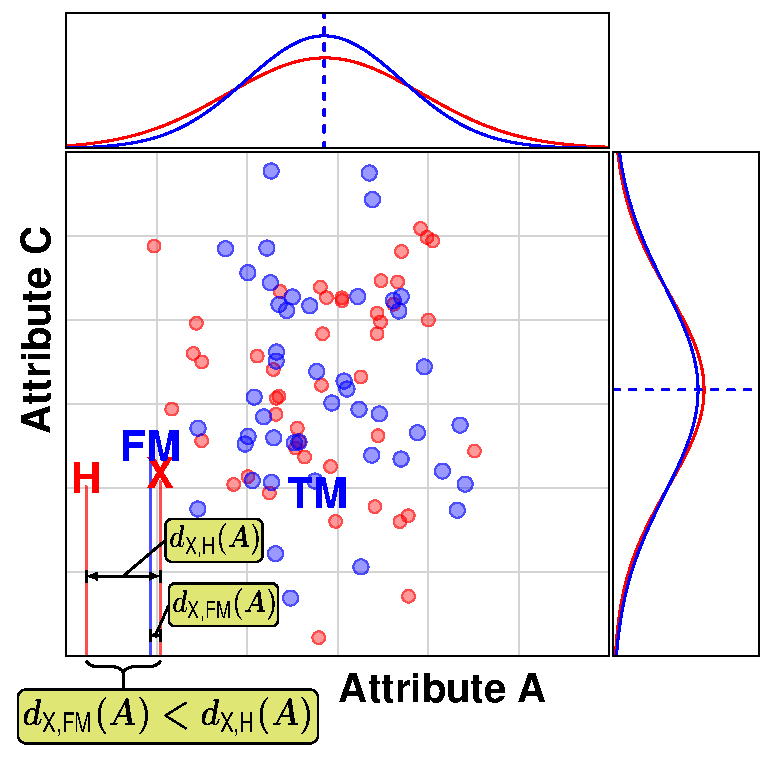
\includegraphics[width=0.8\textwidth]{glmSTIR_figure_2D_final_CvsA.pdf}}
%\end{minipage} \hspace{-0.4cm}
%\begin{minipage}[c]{0.5\textwidth}
%\centering
%\caption{{\bf Imposters vs true neighbors in the presence of interactions with three variables}. Scatter plot of simulated irrelevant Attribute C with a functional Attribute A {\bf(a)}. None of the attributes has a main effect, but Attribute B and C interact through differential correlation {\bf(b)}. Computing nearest neighbors with irrelevant attributes {\bf(a)} or lower dimensions leads to imposter nearest neighbors and degrades the ability of Relief-based methods to identify interaction effects. Computing distances in only these two dimensions leads to an imposter false miss (FM) for the nearest neighbor from the opposite outcome class for target instance X. This imposter leads to attribute A predicting closer projected distances for misses than hits (H), which incorrectly indicates that A is a poor discriminator (yellow boxes in {\bf a}). Computing nearest neighbors in higher dimensions {\bf(c-d)} or with the correct interaction partner leads to imposter nearest neighbor (FM) being replaced by the true nearest miss neighbor (TM) for target instance X, which correctly leads to attribute A predicting closer projected distances for hits (H) than misses, which is an indication that attribute A is a good discriminator (yellow boxes {\bf(b)}).}\label{fig:2dAvC}
%\end{minipage}
%%\end{center}
%\end{figure}

\newpage

\begin{figure}[h!]
\begin{wrapfigure}{l}{0.6\textwidth}
    \vspace{-12pt}
	\centering
	\framebox{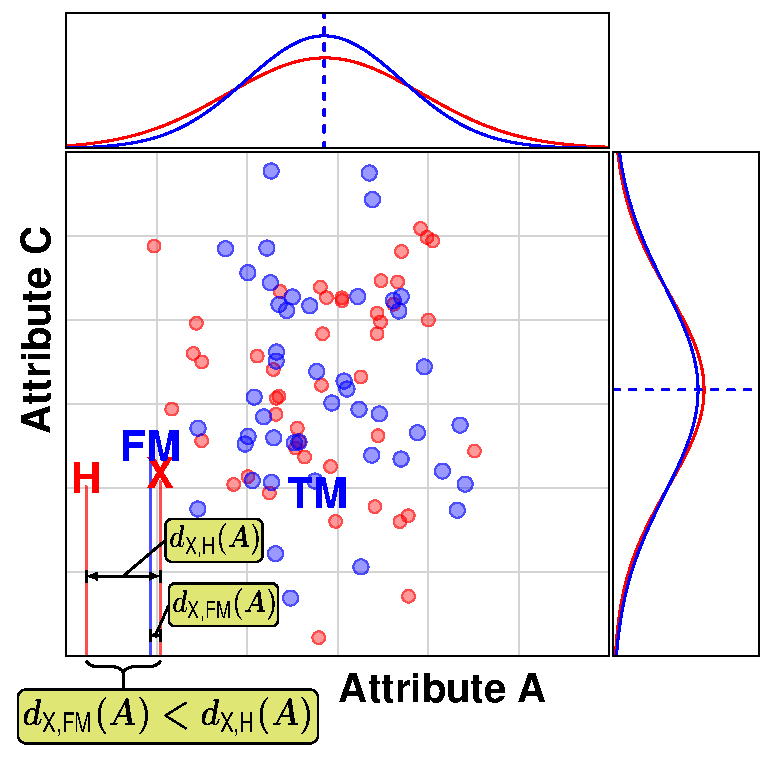
\includegraphics[width=0.55\textwidth]{glmSTIR_figure_2D_final_CvsA.pdf}}
\end{wrapfigure}
\noindent\refstepcounter{figure}\textbf{Fig \thefigure \label{fig:2dAvC}.} \textbf{Imposters vs true neighbors in the presence of interactions with three variables}. Scatter plot of simulated irrelevant Attribute C with a functional Attribute A \textbf{(a)}. None of the attributes has a main effect, but Attribute B and C interact through differential correlation \textbf{(b)}. Computing nearest neighbors with irrelevant attributes \textbf{(a)} or lower dimensions leads to imposter nearest neighbors and degrades the ability of Relief-based methods to identify interaction effects. Computing distances in only these two dimensions leads to an imposter false miss (FM) for the nearest neighbor from the opposite outcome class for target instance X. This imposter leads to attribute A predicting closer projected distances for misses than hits (H), which incorrectly indicates that A is a poor discriminator (yellow boxes in \textbf{(a)}). Computing nearest neighbors in higher dimensions \textbf{(c-d)} or with the correct interaction partner leads to imposter nearest neighbor (FM) being replaced by the true nearest miss neighbor (TM) for target instance X, which correctly leads to attribute A predicting closer projected distances for hits (H) than misses, which is an indication that attribute A is a good discriminator (yellow boxes \textbf{(b)}).
\end{figure}

Relief-based methods use information from all attributes available to it (omnigenic) to estimate an attribute's importance. However, if relevant higher-dimensional information is not used, even Relief-based methods will miss the effect of A because ``imposter'' neighbors will be used in the attribute estimate (False Miss (FM) in Fig.~\ref{fig:2dAvC}, where $d_{\text{X,FM}}(A)<d_{\text{X,H}}(A)$).  If one were to compute nearest neighbors in the A-C plane (ignoring the B dimension), the nearest miss would be an imposter (FM), which leads to a negative contribution to the importance score for A. One might call this C attribute a type-I confounding attribute because it increases the chances of interacting attributes to be false negatives. When nearest neighbors are calculated based on higher dimensions with relevant information (Fig.~\ref{fig:2dAvB}c), it is clear that TM is closer to X than FM. The imposter (FM) is replaced by the true nearest miss (TM) and attribute A correctly shows a greater projected difference between misses than hits (Fig.~\ref{fig:2dAvB}d $d_{\text{X,TM}}(A)>d_{\text{X,H}}(A)$), which is the signature of an important attribute. Univariate methods still cannot find the importance of A unless the interaction is explicitly modeled, but as long as functional variables A and B are in the space for nearest neighbor calculations (Fig.~\ref{fig:2dAvB}c-d), imposters can be excluded and Relief-based methods will find that A (and B) are important discriminators. 

\begin{figure}[h!]
%%\begin{center}
\begin{minipage}[c]{0.4\textheight}
\centering 
		\framebox{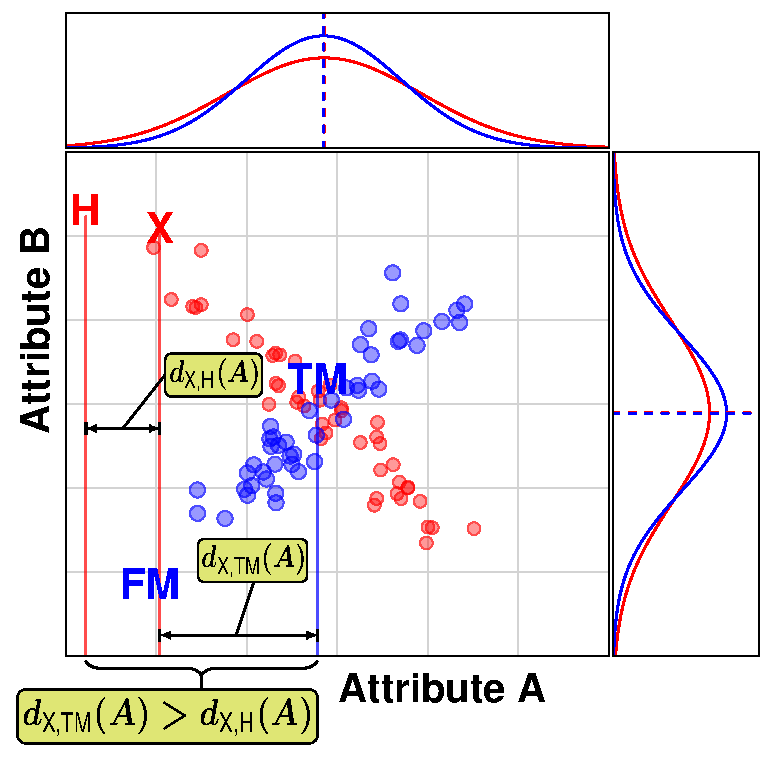
\includegraphics[width=0.8\textwidth]{glmSTIR_figure_2D_final_BvsA.pdf}}
\end{minipage} \hspace{-0.4cm}
\begin{minipage}[c]{0.5\textwidth}
\centering
\caption{{\bf True neighbors}}\label{fig:2dAvB}
\end{minipage}
%%\end{center}
\end{figure}  

\begin{figure}[h!]
%%\begin{center}
\begin{minipage}[c]{0.4\textheight}
\centering
		\framebox{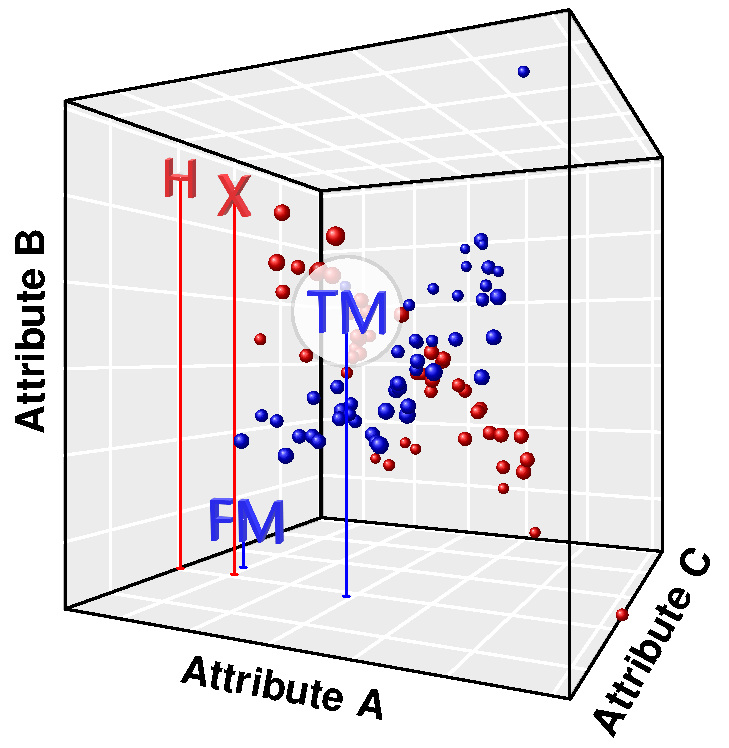
\includegraphics[width=0.8\textwidth]{nice_box_2D_points.pdf}}
\end{minipage} \hspace{-0.4cm}
\begin{minipage}[c]{0.5\textwidth}
\centering
\caption{{\bf 3D AB view}. Still working on this. }\label{fig:3d_c}
\end{minipage}
%%\end{center}
\end{figure}  

\begin{figure}[h!]
%%\begin{center}
\begin{minipage}[c]{0.4\textheight}
\centering
		\framebox{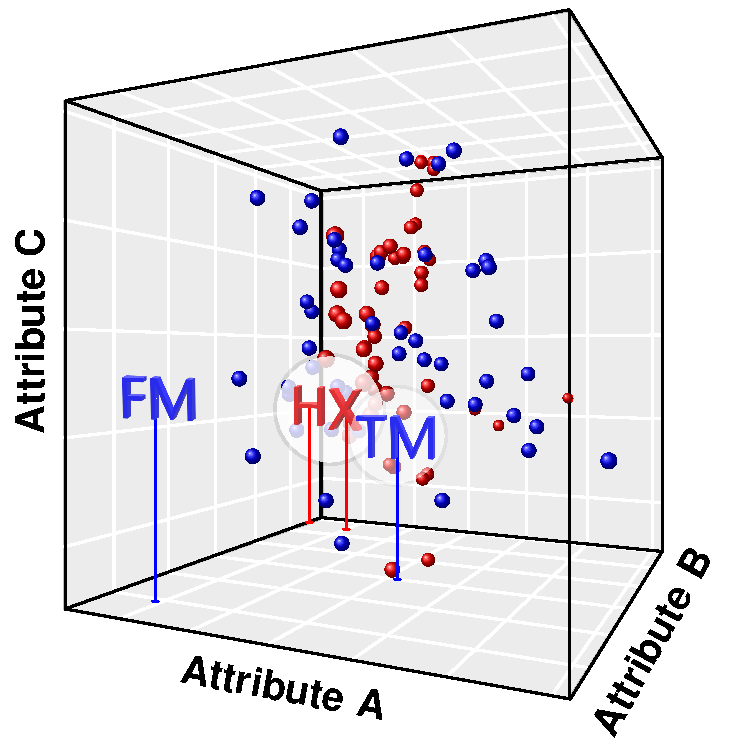
\includegraphics[width=0.8\textwidth]{nice_box_2D_points2.pdf}}
\end{minipage} \hspace{-0.4cm}
\begin{minipage}[c]{0.5\textwidth}
\centering
\caption{{\bf 3D AC view}. Still working on this. }\label{fig:3d_d}
\end{minipage}
%%\end{center}
\end{figure}  

Using same interaction, increase background noise genes to see degrading of A and B Relief importance because of curse of dimensionality (sparseness).  

\bibliography{BoD}   % name of bib file

\end{document}
